\documentclass[11pt]{article}
\setlength\headheight{13.6pt}%
\usepackage[utf8]{inputenc} % Required for inputting international characters
\usepackage[T1]{fontenc} % Output font encoding for international characters
\usepackage{polski}
\usepackage{mathpazo} % Palatino font
\usepackage{graphicx}
\usepackage{fancyhdr}
\usepackage{etoolbox}
\usepackage{blindtext}
\usepackage{geometry}
\geometry{legalpaper, margin=1in}
\usepackage[cleardoublepage=plain]{scrextend}
\graphicspath{ {images/.\ProjectAiMO} } %change to yours path
\pagestyle{fancy}
\fancyhf{}
\rhead{2017/2018}
\lhead{Projekt z Analizy i Modelowania Oprogramowania}
\rfoot{Strona \thepage}
\begin{document}
	
	\begin{titlepage} 
	
		\newcommand{\HRule}{\rule{\linewidth}{0.5mm}} % Defines a new command 
		
		\center % Centre everything on the page
		
		%------------------------------------------------
		%	Nagłówki
		%------------------------------------------------
		
		\textsc{\LARGE Akademia Górniczo-Hutnicza im. Stanisława Staszica w Krakowie}\\[1.5cm] % Main heading such as the name of your university/college
		
		\textsc{\Large Projekt z Analizy i Modelowania Oprogramowania}\\[0.5cm] % Major heading such as course name
		
		\textsc{\large Informatyka EAIiIB 2017/2018}\\[0.5cm] % Minor heading such as course title
		
		%------------------------------------------------
		%	Tytuł
		%------------------------------------------------
		
		\HRule\\[0.4cm]
		
		{\huge\bfseries Automat do sprzedaży zakąsek}\\[0.4cm] % Title of your document
		
		\HRule\\[1.5cm]
		
		%------------------------------------------------
		%	Authorzy
		%------------------------------------------------
		
		\begin{minipage}{0.4\textwidth}
			\begin{flushleft}
				\large
				\textit{Autorzy}\\
				Jakub \textsc{Kacorzyk} \\
				Bartłomiej \textsc{Łazarczyk}
			\end{flushleft}
		\end{minipage}
		~
		\begin{minipage}{0.4\textwidth}
			\begin{flushright}
				\large
				\textit{Prowadzący}\\
				dr inż. Wojciech \textsc{Szmuc} % Supervisor's name
			\end{flushright}
		\end{minipage}
		
		%------------------------------------------------
		%	Logo
		%------------------------------------------------
		
		\vfill
		
\includegraphics[scale=1.0]{logo.jpg}
		
		%------------------------------------------------
		%	Data
		%------------------------------------------------
		
		\vfill\vfill\vfill % Position the date 3/4 down the remaining page
		
		{\large\today} 
		
		%----------------------------------------------------------------------------------------
		
		\vfill % Push the date up 1/4 of the remaining page
		
	\end{titlepage}
	
	\tableofcontents
	\cleardoublepage
	\setcounter{page}{2}
	
	\section{Streszczenie projektu}
			Celem naszego projektu jest zamodelowanie automatu do sprzedaży zakąsek.
			
			System oczekując na reakcje z zewnątrz wyświetla na panelu dotykowym wraz z wyświetlaczem prośbę o wybranie produktu. Następnie klient podaje numer produktu, który chciałby zakupić w wyniku czego system sprawdza dostępność danego produktu oraz jego cenę w bazie. W przypadku braku produktu wyświetlana jest komunikat o braku produktu lub złym numerze. Gdy dany produkt jest dostępny, wyświetlana  jest informacja o cenie produktu oraz o metodach sposobu zapłaty. Klient może wybrać płatność gotówką bądź też kartą.
			
			W przypadku wyboru płatności gotówką wyświetlany jest komunikat o wrzuceniu monety. Wrzucona moneta jest sprawdzana przez system obsługi gotówki i w razie niepowodzenia jest wyrzucana z powrotem. W przypadku prawidłowego wyniku sprawdzenia, wartość monety jest odliczana. Następnie sprawdzane jest czy osiągnięto dokładnie kwotę ceny produktu. Jeżeli suma jest mniejsza od ceny proces jest powtarzany. Gdy wrzucona suma jest większa lub równa cenie następuje wydanie produktu oraz reszty. Wydanie reszty jest możliwe, gdy odpowiednia ilość bilonów jest w zbiorniku, w przeciwnym wypadku automat informuję o braku możliwości wydania reszty oraz zwraca wpłacone pieniądze. Możliwe jest też anulowanie zakupu, w wyniku czego wydawana jest cała kwota wpłacona do automatu oraz kończony jest proces zakupu.
			
			W przypadku wyboru płatności kartą, główny system przekazuje żądanie rozpoczęcia transakcji do terminala, będącego osobnym systemem. Główny system otrzymuje informację o pozytywnym bądź negatywnym przebiegu transakcji. W przypadku pozytywnego przebiegu zostaje wyświetlony komunikat o zapłaceniu oraz wydawany jest produkt. W przypadku negatywne przebiegu, cały proces zakupy zostaje anulowany oraz wyświetlany jest komunikat o braku zapłaty.
			
			Automat ma również przygotowany system obsługi automatu przez osobę serwisującą. Ma ona dostęp do drzwi automatu i jest w stanie je otworzyć. System wykrywa takie zachowanie i wyświetla w danym momencie informację, że drzwi zostały otwarte. Następnie serwisant może wypłacić gotówkę, uzupełnić automat, bądź też zmienić produkt w automacie. W przypadku wyboru wypłaty gotówki, system otwiera zbiornik na bilony oraz wyświetla komunikat o zamknięciu zbiornika po wyciągnięciu pieniędzy. Gdy zbiornik zostaje zamknięty, system wyświetla komunikat o zakończeniu wypłaty gotówki. W przypadku wyboru uzupełnienia automatu
			w produkty, system wyświetla informację o uzupełnianiu podczas tego procesu oraz wyświetla informację o zakończeniu uzupełniania po zakończeniu całego procesu. W przypadku wyboru zmiany produktu, system wyświetla komunikat i wyborze numeru produktu, który ma zostać zmieniony. Następnie system prosi o wprowadzenie nowej kwoty produktu, po czym jest sprawdzana jej poprawność. W przypadku pozytywnego sprawdzenia cena produktu jest aktualizowana. W przypadku wykrytej nieprawidłowości w podanej kwocie, wyświetlany jest komunikat o niepoprawności kwoty, a cały proces rozpoczynany jest od nowa.  
			
	\newpage
    \section{Diagram użyć.}
		\begin{center}
			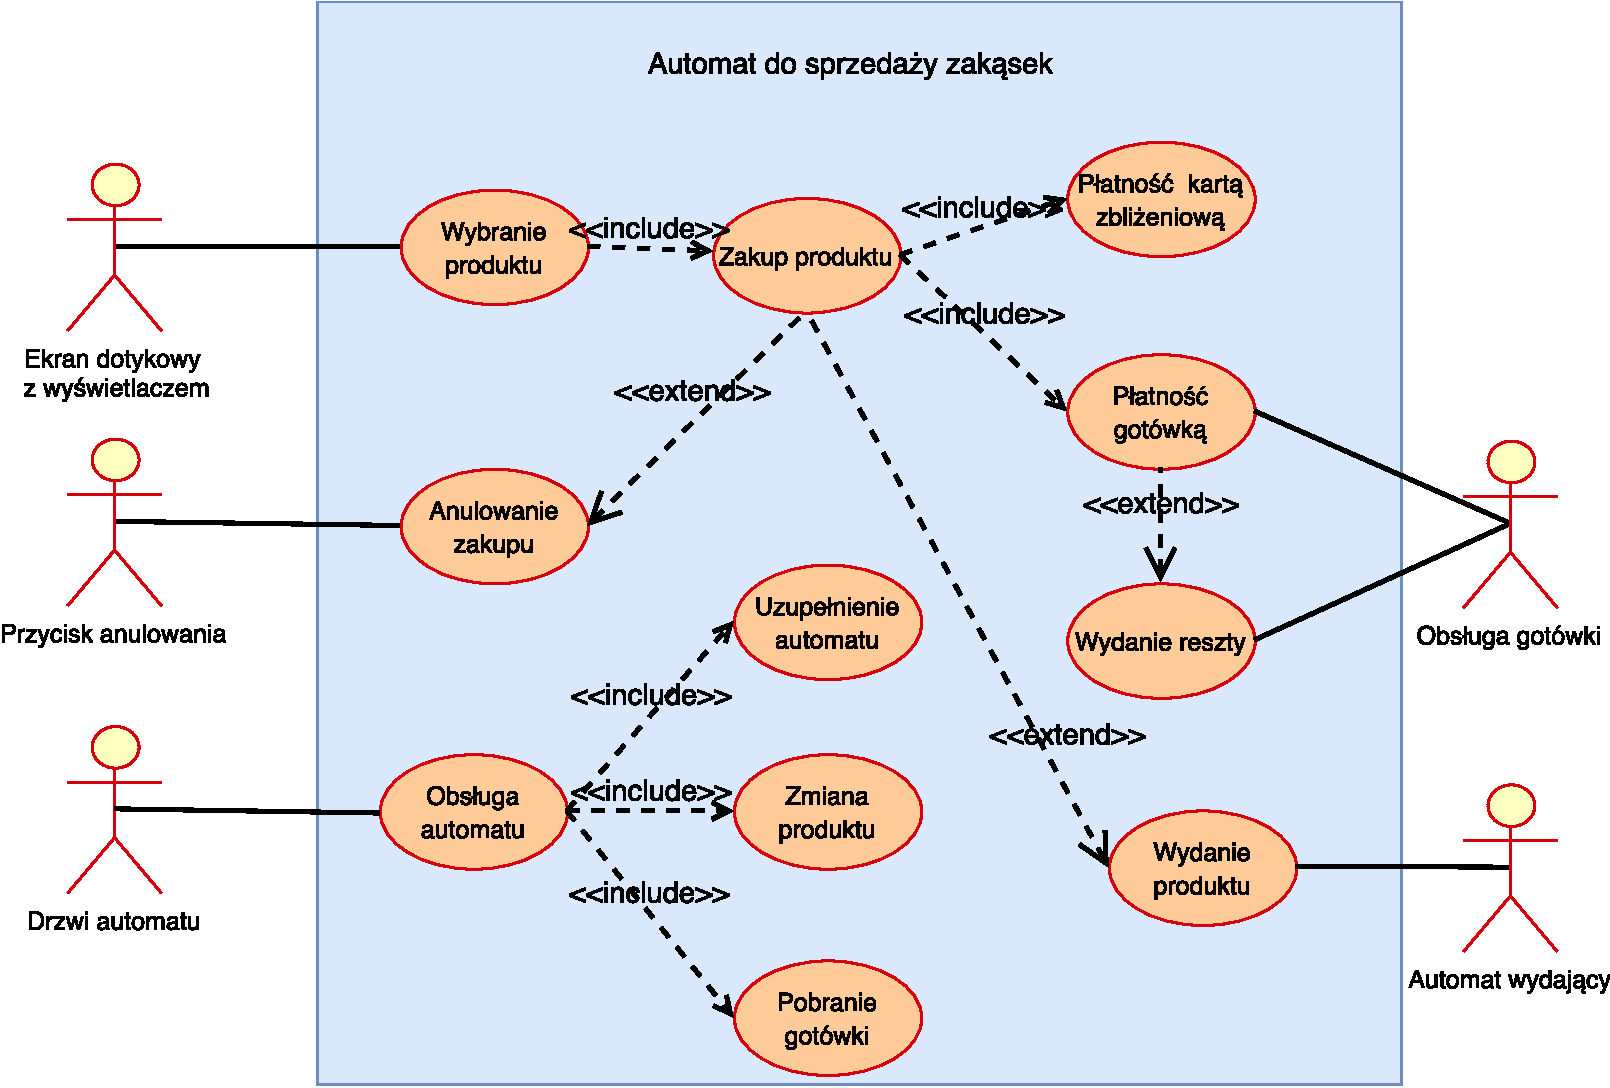
\includegraphics[scale=0.65]{UseCaseDiagram.pdf}
		\end{center}
		\newpage
	\section{Diagramy sekwencji.}
		\subsection{Wybieranie produktu udane.}
		\begin{center}
			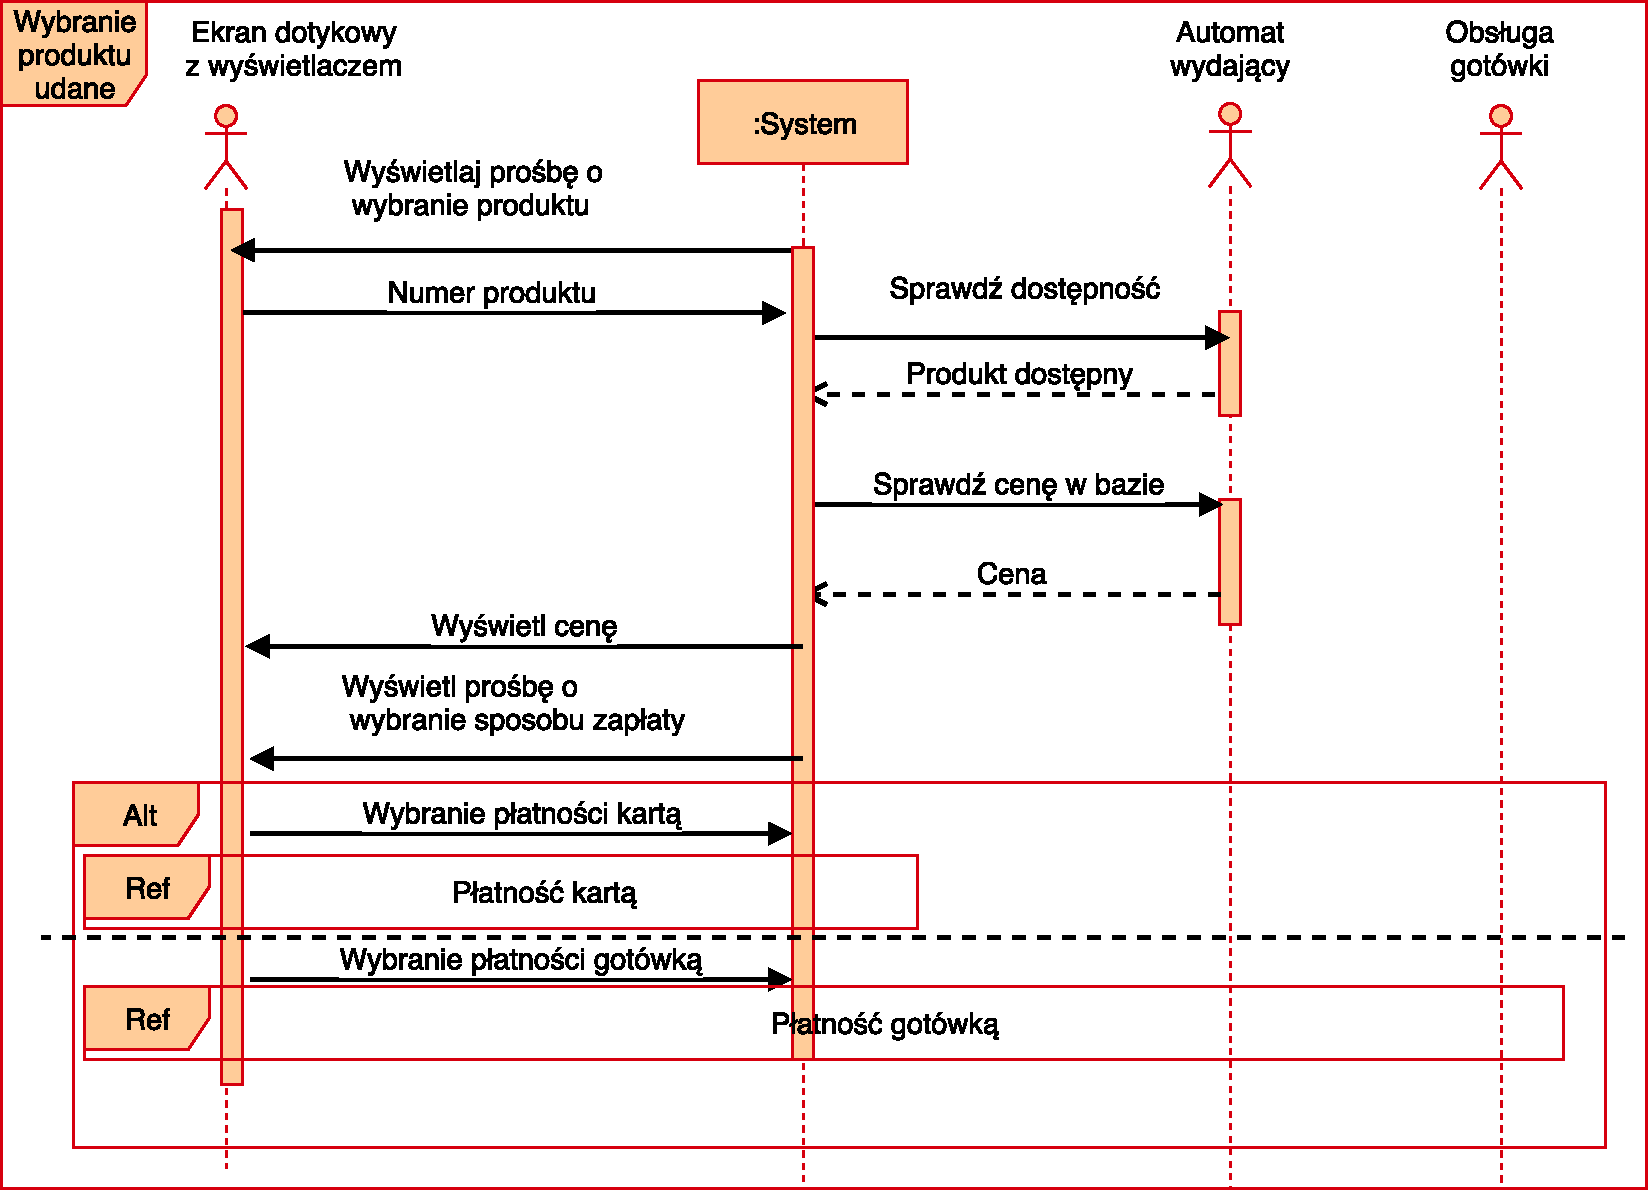
\includegraphics[scale=0.65]{WybranieProduktuUdane.pdf}
		\end{center}
		\subsection{Wybranie produktu nieudane.}
		\begin{center}
			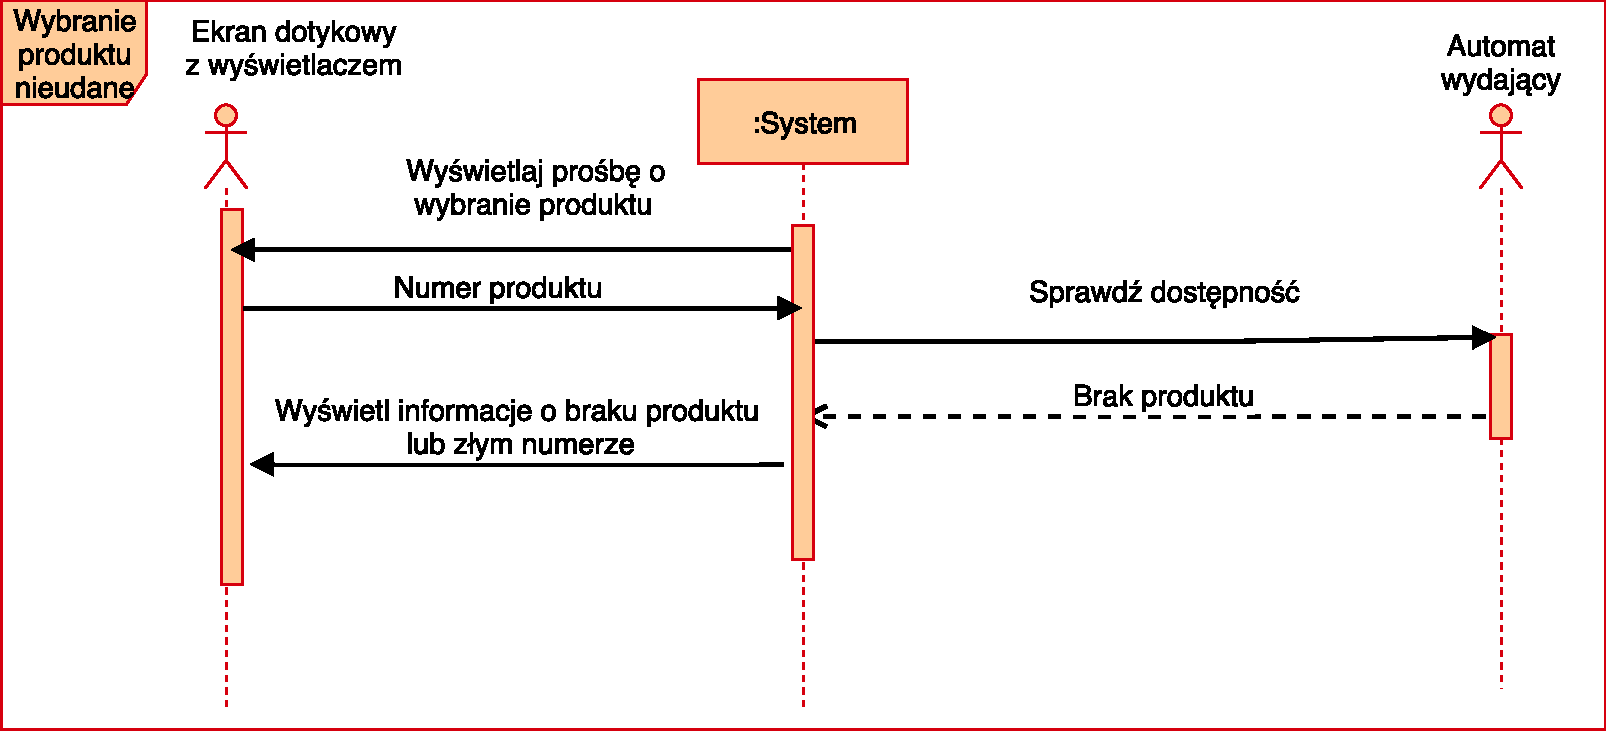
\includegraphics[scale=0.65]{WybranieProduktuNieudane.pdf}
		\end{center}
		\newpage
		\subsection{Płatność kartą udana.}
		\begin{center}
			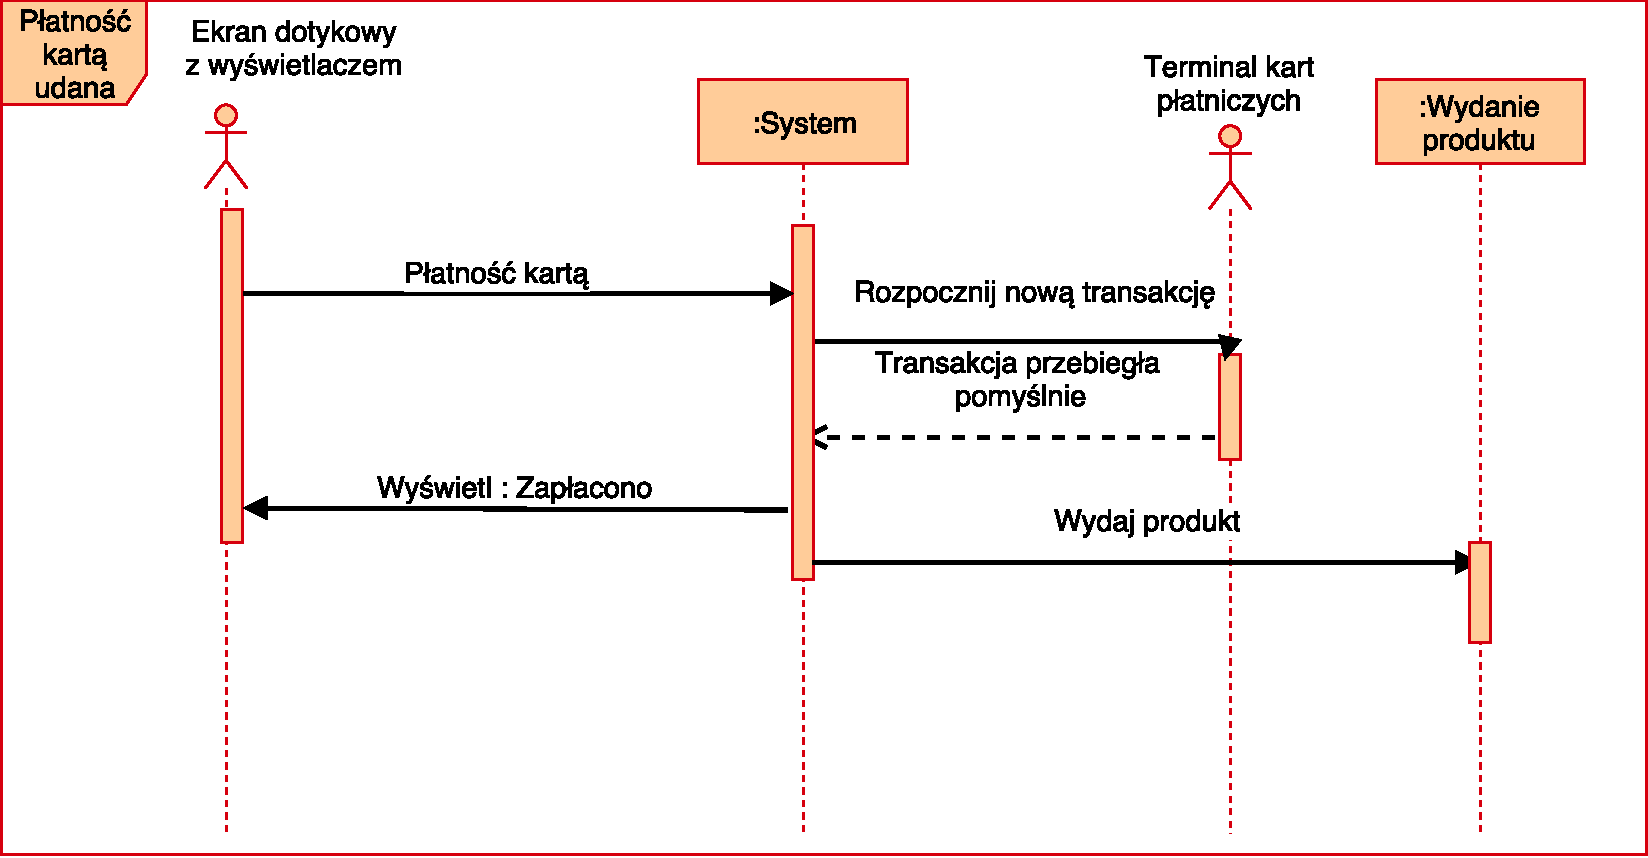
\includegraphics[scale=0.65]{PlatnoscKartaUdana.pdf}
		\end{center}
		\subsection{Płatność kartą nieudana.}
		\begin{center}
			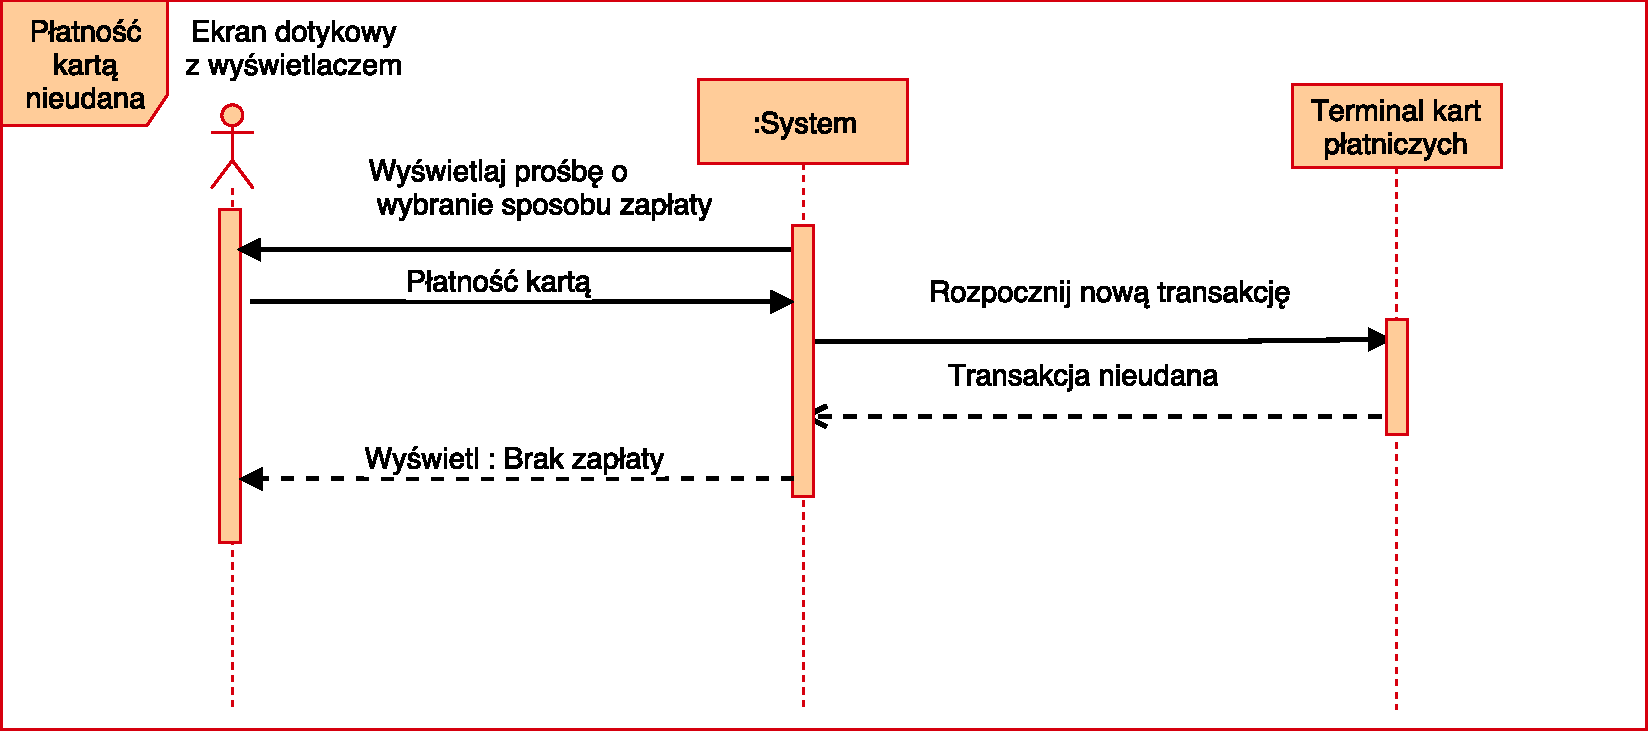
\includegraphics[scale=0.65]{PlatnoscKartaNieudana.pdf}
		\end{center}
		\newpage
		\subsection{Płatność gotówką udana.}
		\begin{center}
			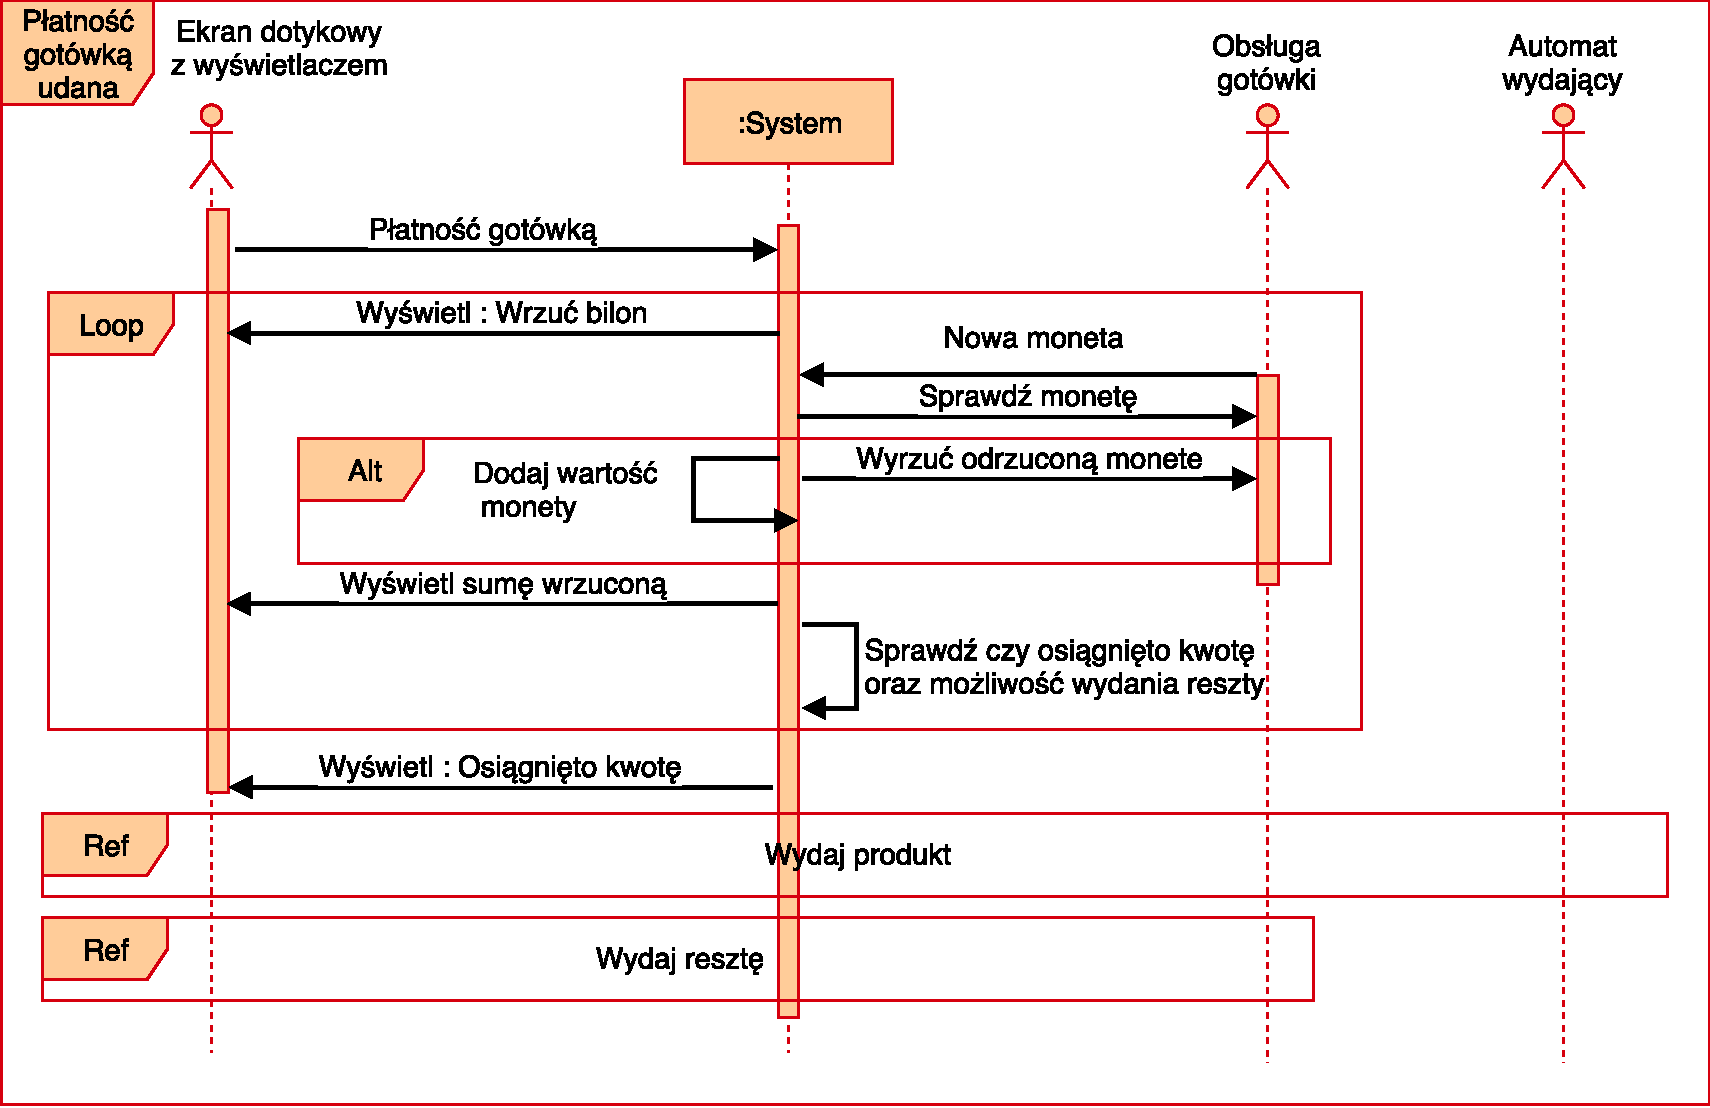
\includegraphics[scale=0.60]{PlatnoscGotowkaUdana.pdf}
		\end{center}
		\subsection{Płatność gotówką nieudana.}
		\begin{center}
			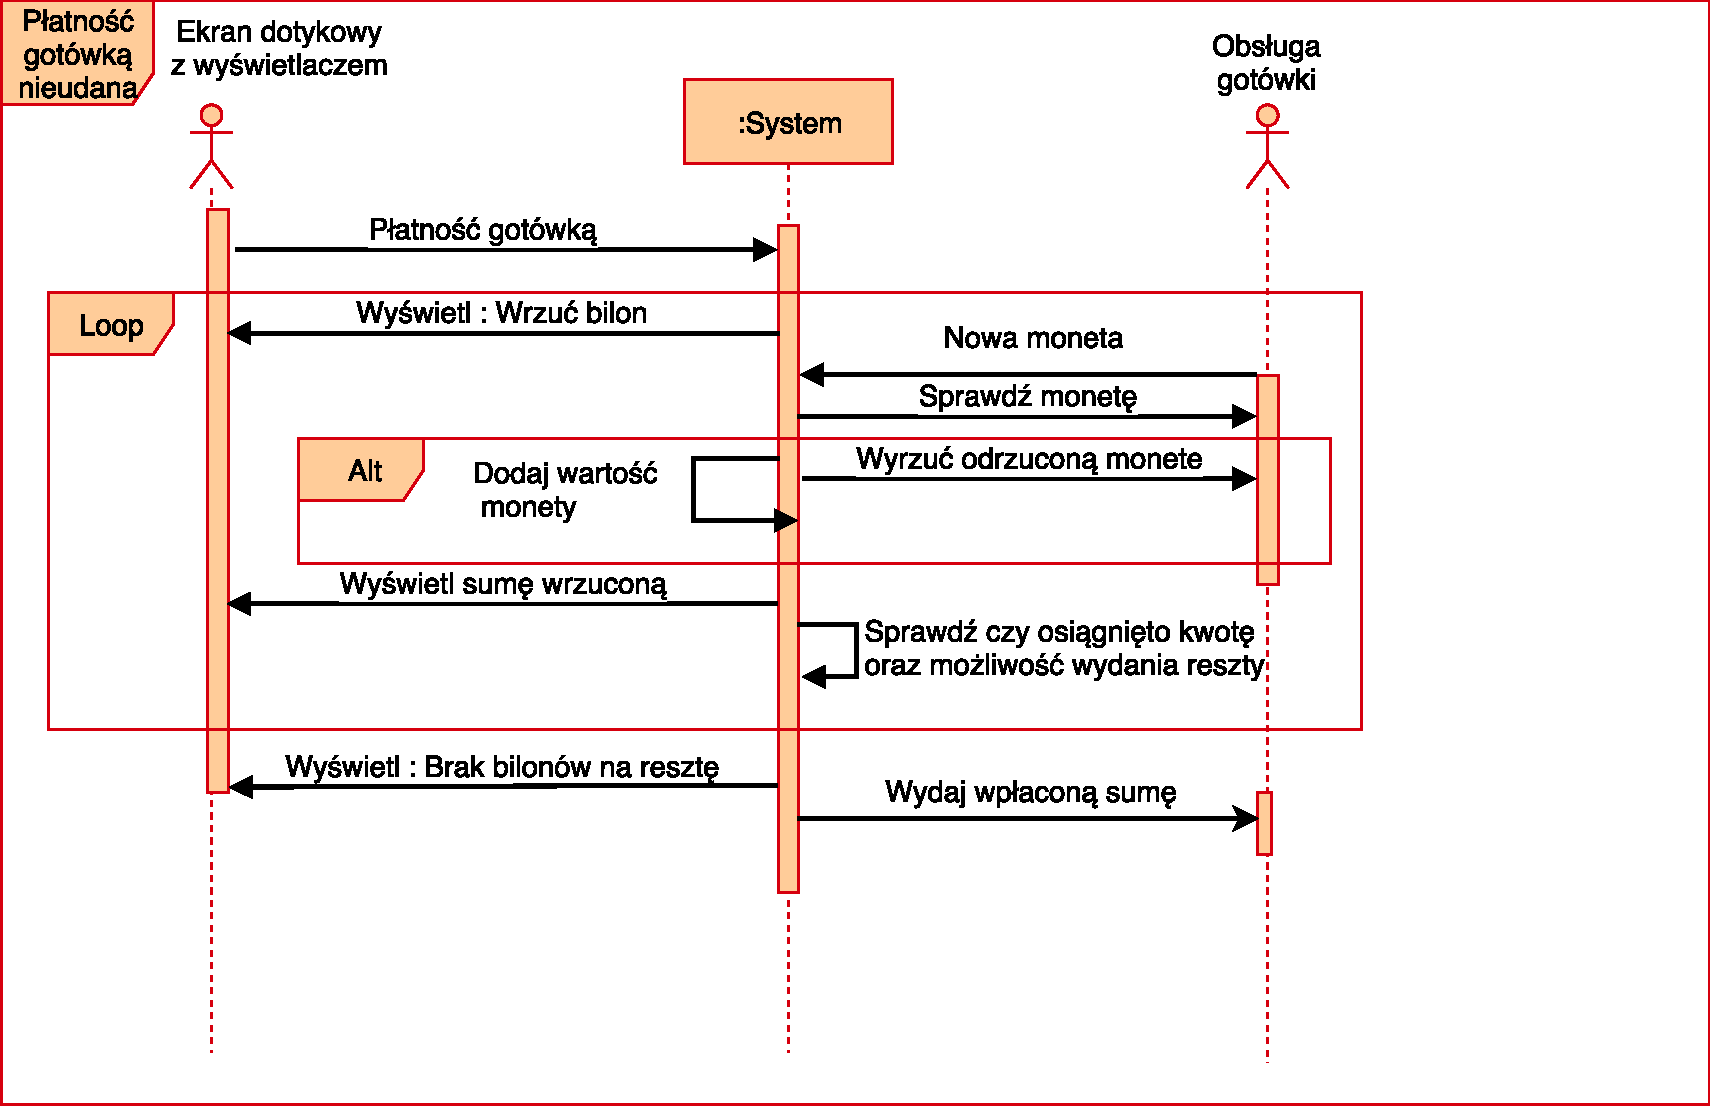
\includegraphics[scale=0.60]{PlatnoscGotowkaNieudana.pdf}
		\end{center}
		\newpage
		\subsection{Wydanie produktu.}
		\begin{center}
			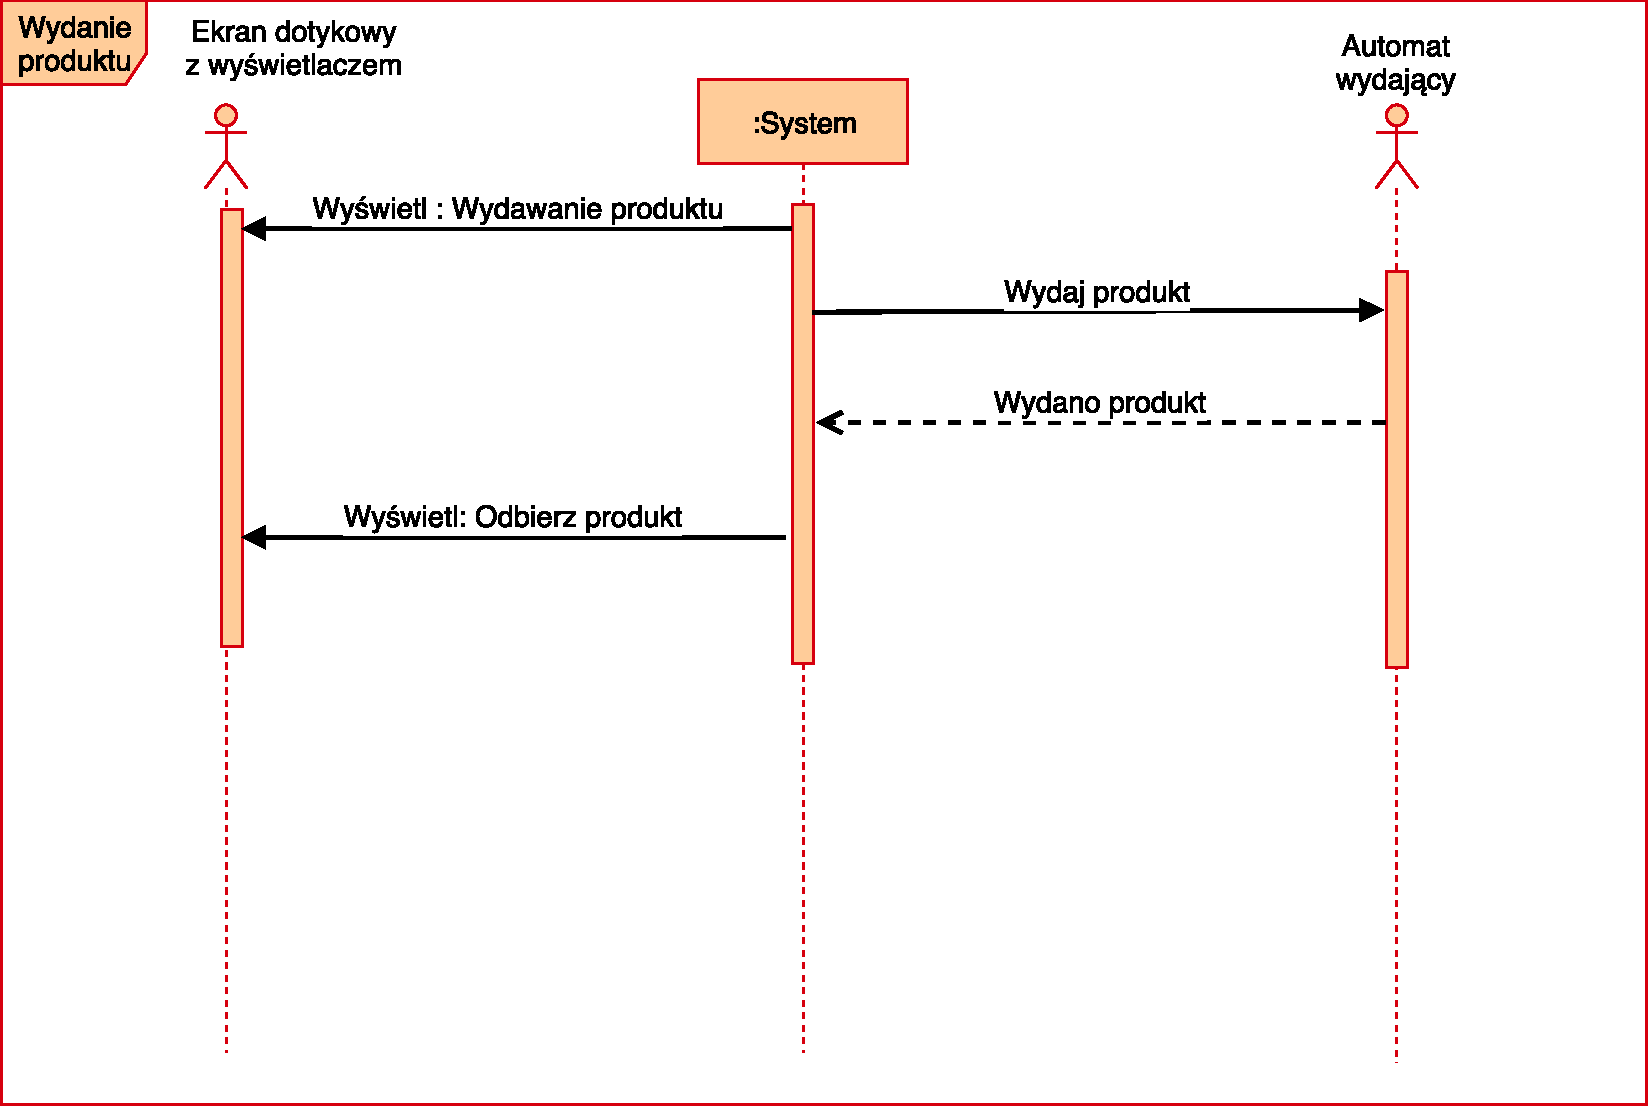
\includegraphics[scale=0.65]{WydanieProduktu.pdf}
		\end{center}
		\newpage
		\subsection{Wydanie reszty.}
		\begin{center}
			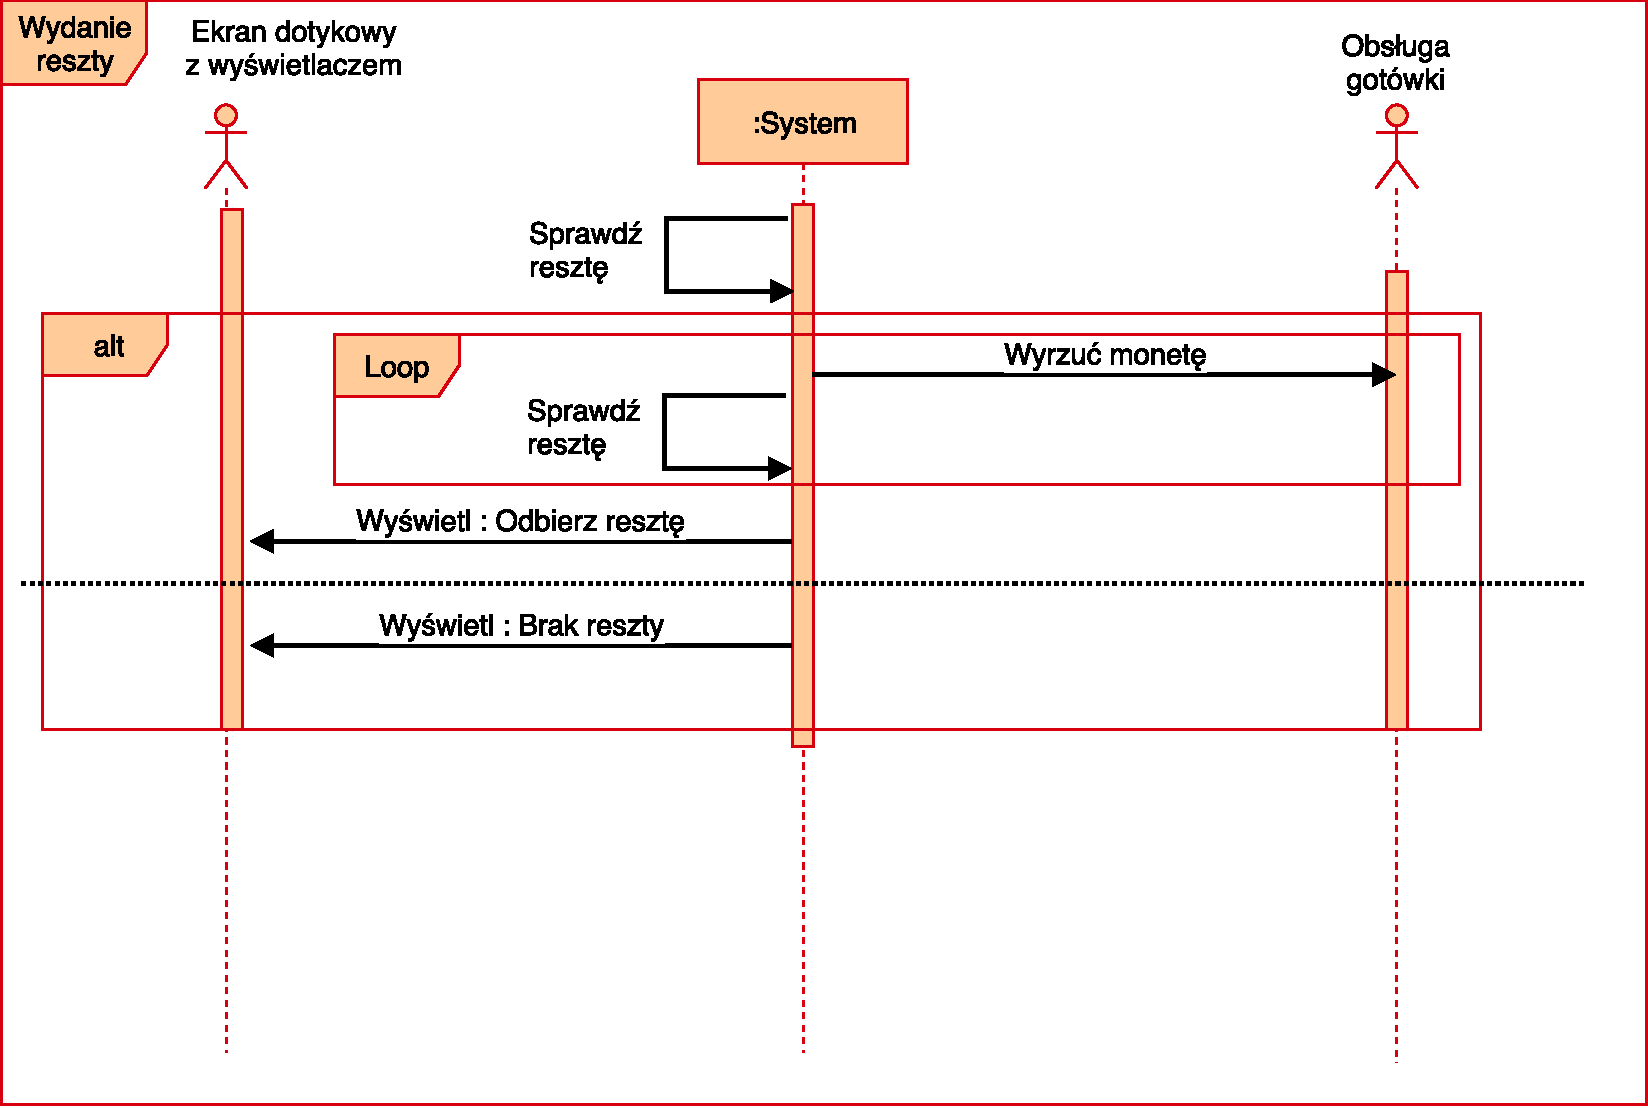
\includegraphics[scale=0.65]{WydanieReszty.pdf}
		\end{center}
		\newpage
		\subsection{Anulowanie zakupu.}
		\begin{center}
			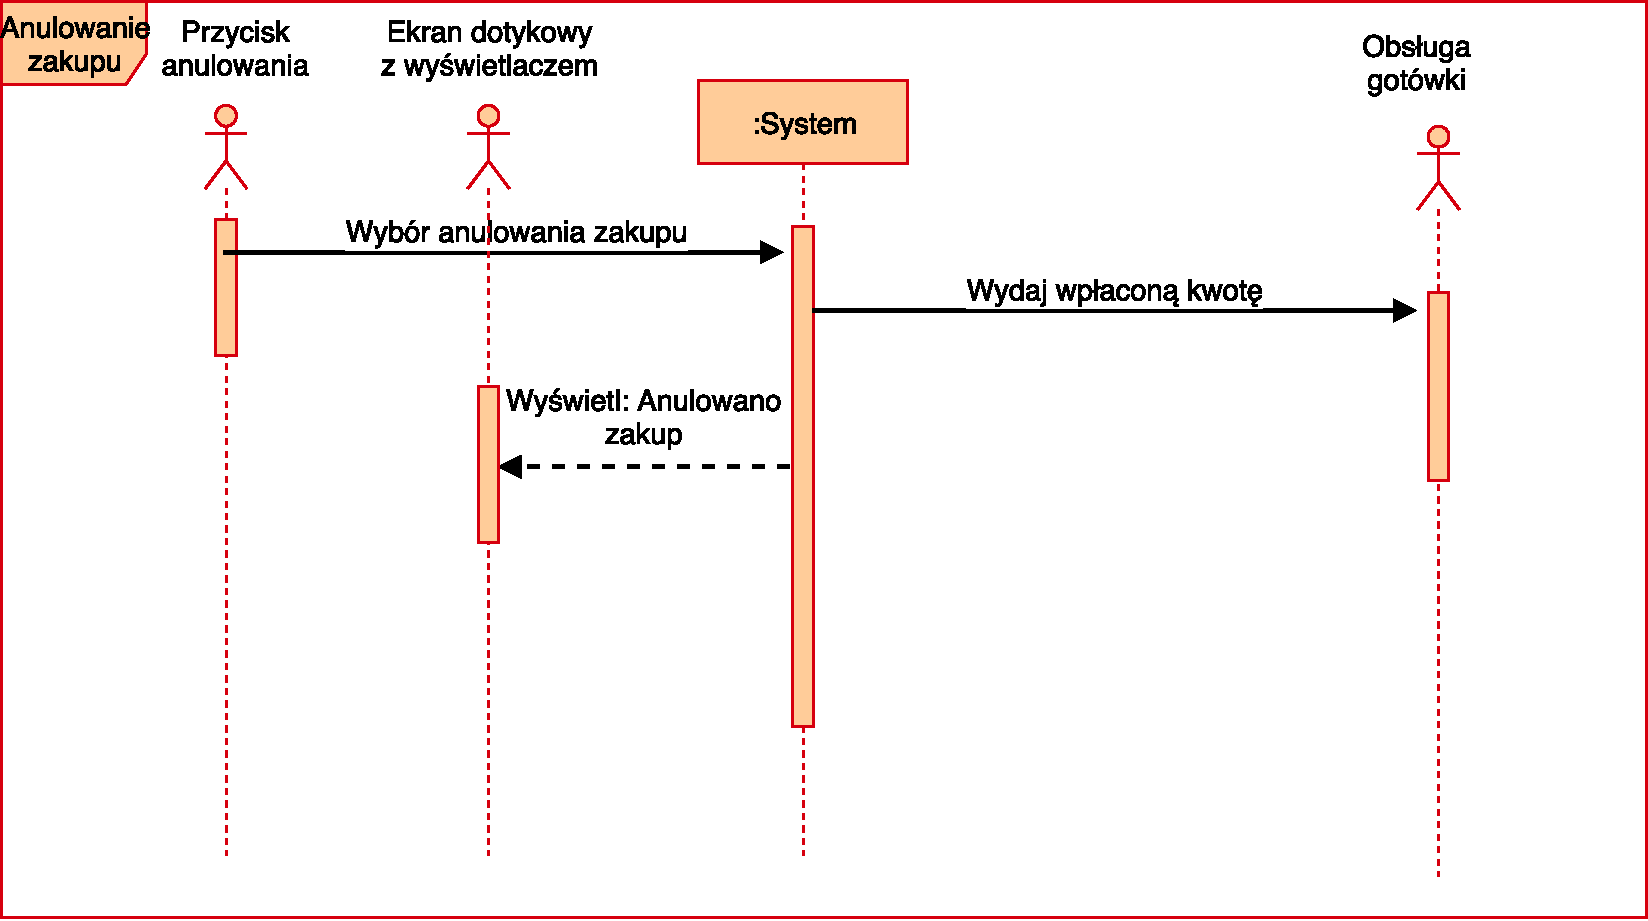
\includegraphics[scale=0.65]{AnulowanieZakupu.pdf}
		\end{center}
		\newpage
		\subsection{Obsługa automatu.}
		\begin{center}
			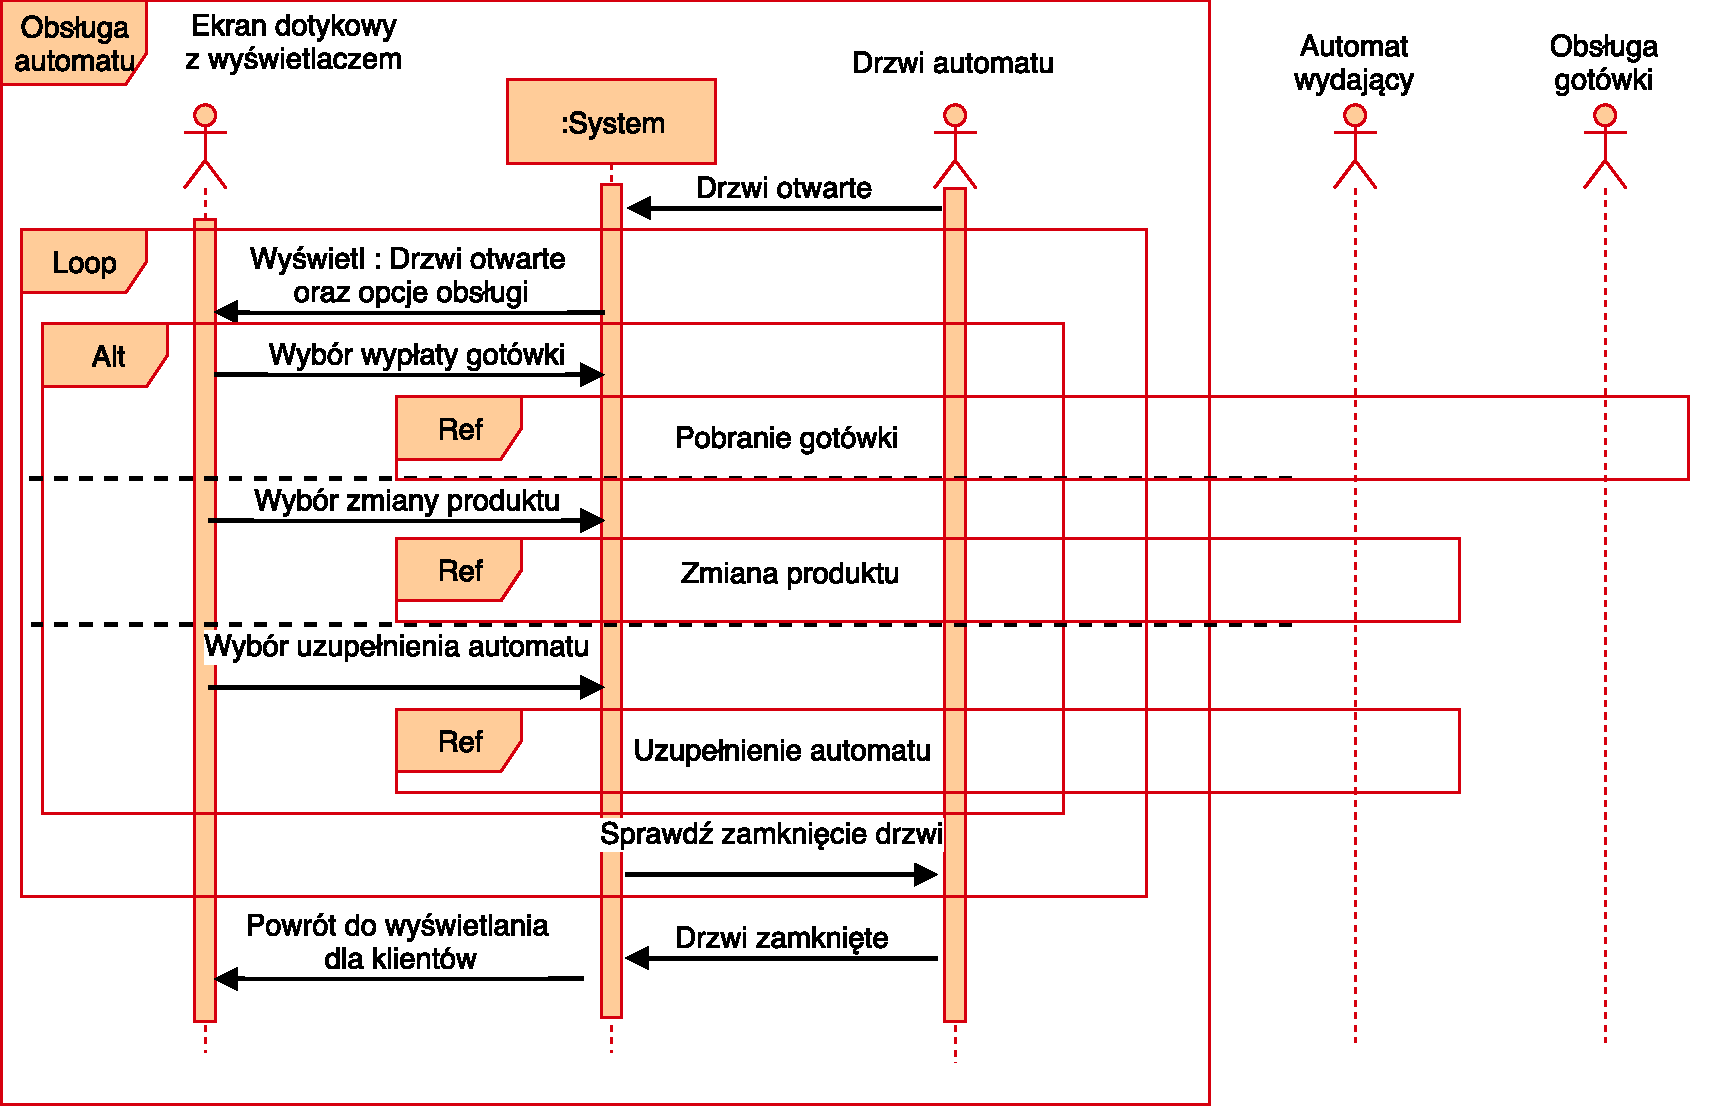
\includegraphics[scale=0.65]{ObslugaAutomatu.pdf}
		\end{center}
		\newpage
		\subsection{Pobranie gotówki.}
		\begin{center}
			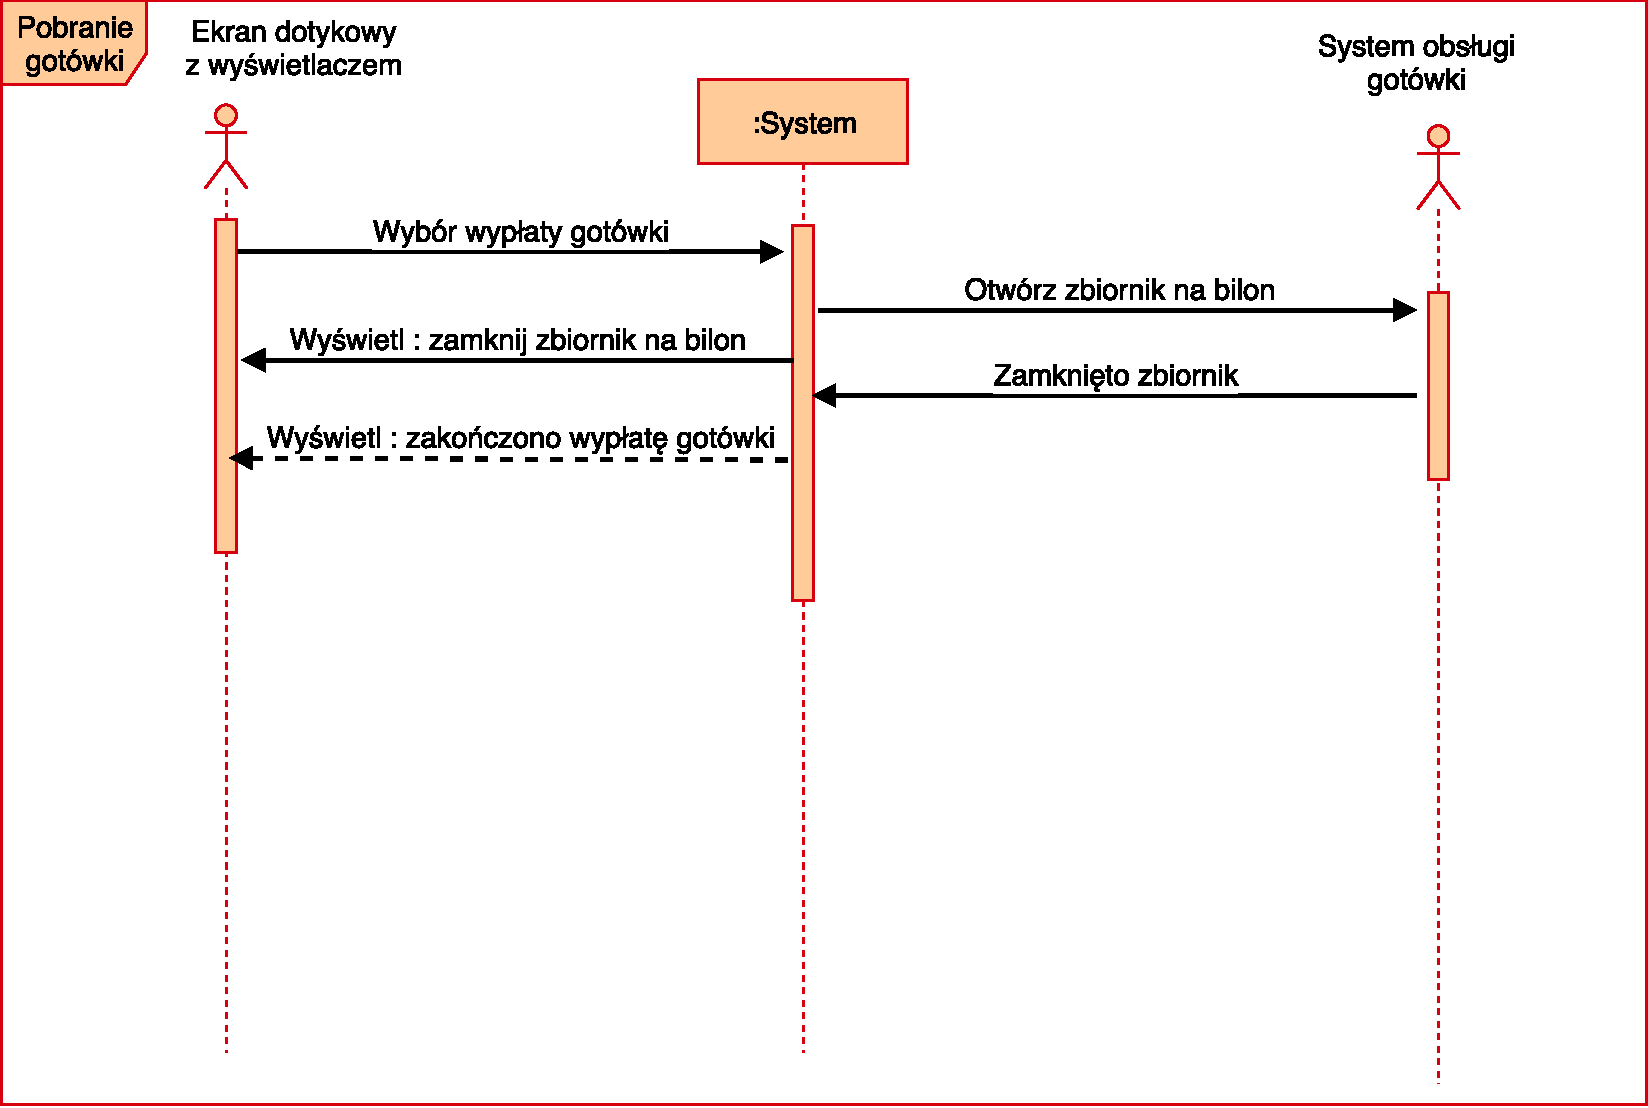
\includegraphics[scale=0.65]{PobranieGotowki.pdf}
		\end{center}
		\newpage
		\subsection{Uzupełnienie automatu.}
		\begin{center}
			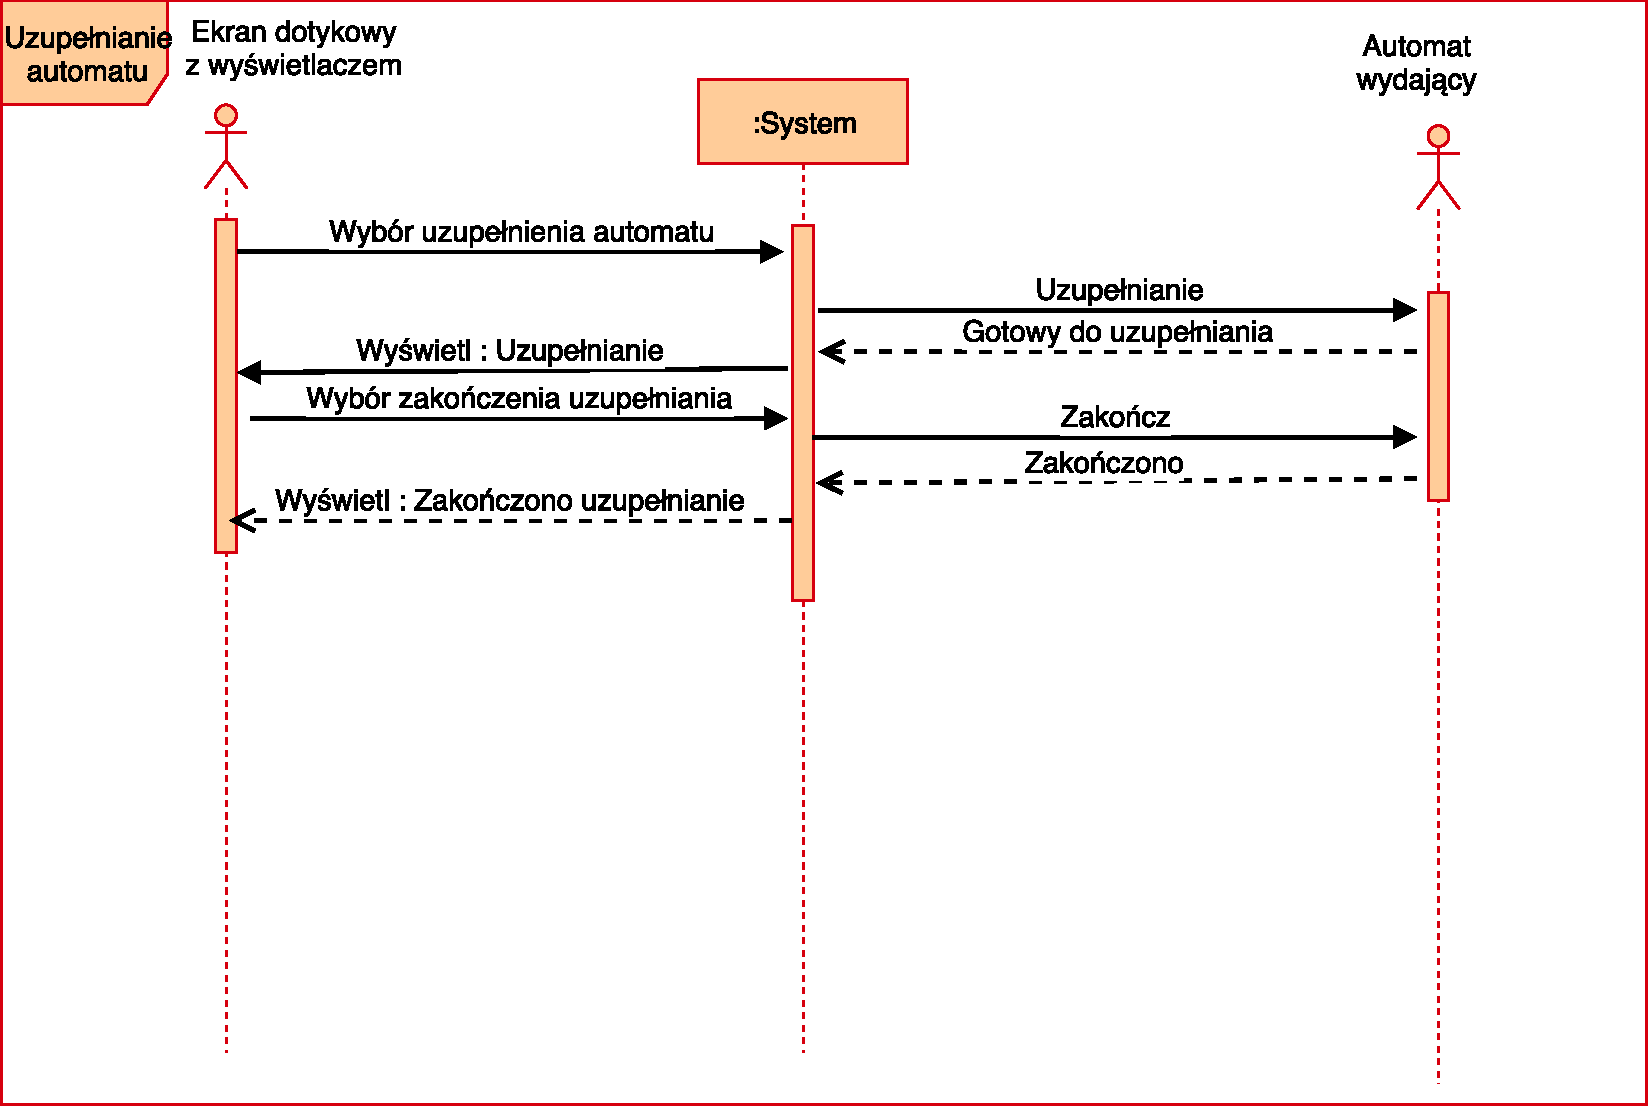
\includegraphics[scale=0.65]{UzupelnianieAutomatu.pdf}
		\end{center}
		\newpage
		\subsection{Zmiana produktu.}
		\begin{center}
			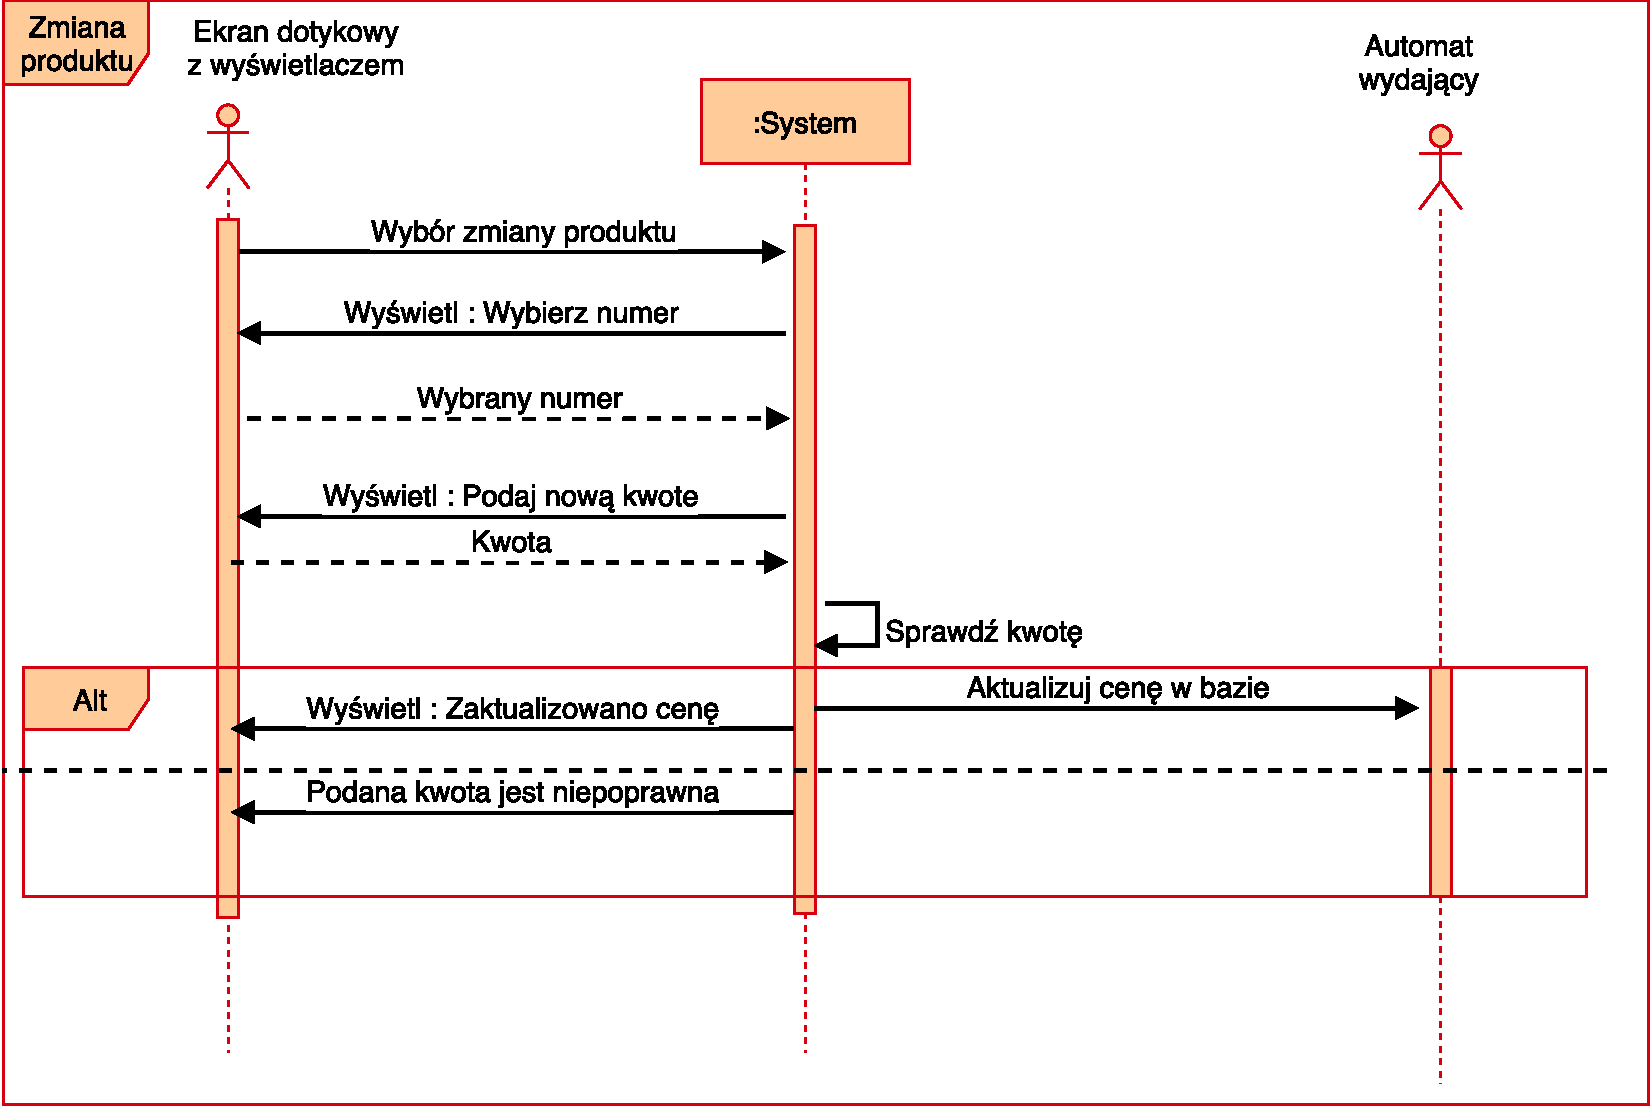
\includegraphics[scale=0.65]{ZmianaProduktu.pdf}
		\end{center}
	\end{document}